% 〈表題〉（技術報告）
% ビルド: tectonic -X compile paper.tex
% 和文フォントに macOS のヒラギノを使うので、macOS でビルドする。欧文と数式のフォントは Tectonic の配布物から読む。
% 〈〉で囲んだ箇所と大文字の仮の名前（REPO、PATH）を書き換え、使わない節と図は消す。
% \code{} の中は ASCII だけにする。url 系の命令は和文フォントへ切り替わらず、和文の文字が欠ける。
\documentclass[xelatex,ja=standard,a4paper,twocolumn,10pt]{bxjsarticle}

% bxjsarticle は geometry を読み込み済みなので、\usepackage ではなく \geometry で指定する
\geometry{top=20mm,bottom=24mm,left=19mm,right=19mm,columnsep=7mm}
\usepackage{amsmath}
\usepackage{unicode-math}
% 欧文は Source の系統でそろえる。Source Serif は同じ 10pt ではヒラギノ明朝より大きく見えるので縮める
\setmainfont{SourceSerifPro}[Extension=.otf,UprightFont=*-Regular,BoldFont=*-Semibold,ItalicFont=*-RegularIt,BoldItalicFont=*-SemiboldIt,Scale=0.94]
\setsansfont{SourceSansPro}[Extension=.otf,UprightFont=*-Regular,BoldFont=*-Semibold,ItalicFont=*-RegularIt,BoldItalicFont=*-SemiboldIt]
\setmonofont{SourceCodePro}[Extension=.otf,UprightFont=*-Regular,BoldFont=*-Semibold,Scale=0.88]
\setmathfont{STIXTwoMath-Regular.otf}[Scale=0.96]
% zxjatype の命令は、オプションをフォント名の前に置く
\setjamainfont[BoldFont=HiraMinProN-W6]{HiraMinProN-W3}
\setjasansfont[BoldFont=HiraginoSans-W6]{HiraginoSans-W3}

\usepackage{graphicx}
\usepackage{xcolor}
\usepackage{booktabs}
\usepackage{tabularx}
\usepackage{array}
\usepackage{enumitem}
\usepackage{fancyvrb}
\usepackage{tikz}
\usetikzlibrary{arrows.meta,calc}
\usepackage{pgfplots}
\pgfplotsset{compat=1.18}
\usepackage[font=small,labelsep=quad,labelformat=simple]{caption}
\captionsetup[table]{position=top,skip=4pt}
\captionsetup[figure]{skip=6pt}
\usepackage[colorlinks=true,linkcolor=linkc,citecolor=linkc,urlcolor=linkc]{hyperref}
\usepackage{xurl}
% 表の数値は S 列で小数点の位置をそろえる。数値でないセル（見出しなど）は {} で包む。
% 数字は周りの文字と同じ書体で組む（既定の数式フォントだと、表の sans と字形が混ざる）
\usepackage{siunitx}
\sisetup{mode=match,reset-text-family=false,reset-text-series=false,reset-text-shape=false}

\definecolor{linkc}{RGB}{29,80,140}
% 本報告で作ったもの、強調したい系列に使う色
\definecolor{ours}{RGB}{194,78,25}
\definecolor{accentc}{RGB}{29,95,166}
\definecolor{warnc}{RGB}{180,35,24}
\definecolor{seriesA}{RGB}{138,147,159}
\definecolor{seriesB}{RGB}{47,109,181}

% 識別子は URL と同じ扱いにして、下線やスラッシュのところで折り返せるようにする。
% url 系の命令はキャプションの中で展開されると壊れるので、robust な命令で包む
\DeclareUrlCommand\codeurl{\urlstyle{tt}}
\DeclareRobustCommand{\code}{\codeurl}

\setlist{nosep,leftmargin=1.4em,topsep=3pt,itemsep=1pt}
\setlength{\emergencystretch}{3em}
\renewcommand{\arraystretch}{1.18}
\newcolumntype{Y}{>{\raggedright\arraybackslash}X}
\newcolumntype{R}{>{\raggedleft\arraybackslash}X}

% 図の共通の描き方。figure* の図は [x=0.2mm,y=-0.2mm] で、幅 820 までの格子に描く（16.4 cm）
\tikzset{
  rb/.style={draw=black!70,fill=white,rounded corners=1pt,line width=0.4pt},
  ro/.style={draw=ours,fill=ours!8,rounded corners=1pt,line width=0.8pt},
  rw/.style={draw=warnc,fill=warnc!6,rounded corners=1pt,line width=0.6pt},
  rg/.style={draw=black!45,dashed,rounded corners=2pt,line width=0.4pt},
  rd/.style={draw=black!50,dashed,fill=white,rounded corners=1pt,line width=0.4pt},
  rp/.style={draw=accentc,fill=accentc!8,line width=0.5pt},
  arr/.style={-{Stealth[length=1.7mm,width=1.3mm]},line width=0.45pt},
  arro/.style={arr,draw=ours,line width=0.8pt},
  arrw/.style={arr,draw=warnc,line width=0.7pt,dashed},
  arrd/.style={arr,draw=black!55,dashed},
  M/.style={anchor=base,inner sep=0pt},
  S/.style={anchor=base west,inner sep=0pt},
  E/.style={anchor=base east,inner sep=0pt},
  t/.style={font=\sffamily\footnotesize},
  tb/.style={font=\sffamily\footnotesize\bfseries},
  ts/.style={font=\sffamily\scriptsize,text=black!70},
  tt/.style={font=\ttfamily\scriptsize},
  tts/.style={font=\ttfamily\fontsize{7}{8.4}\selectfont,text=black!70},
  to/.style={font=\sffamily\footnotesize\bfseries,text=ours},
  tw/.style={font=\sffamily\scriptsize,text=warnc},
}

\begin{document}

\twocolumn[{%
\begin{center}
{\sffamily\small 技術報告\quad 〈作成日 YYYY-MM-DD〉\par}
\vspace{3mm}
{\sffamily\bfseries\LARGE 〈表題。何を、何で、どうしたか〉\par}
\vspace{3mm}
{\itshape\normalsize 〈English title〉\par}
\vspace{3mm}
% 所有者の名前、コミットのハッシュ、誰が何をもとに作ったかは書かない。報告書だけで読めるようにする
{\small\sffamily
対象: \code{REPO} の \code{PATH/}\\
期間: 〈YYYY-MM-DD〉〜〈MM-DD〉\par}
\end{center}
\vspace{1mm}
\noindent\colorbox{black!4}{\parbox{\dimexpr\textwidth-2\fboxsep}{\small
\vspace{1.5mm}
{\sffamily\bfseries 概要}\quad
〈目的を 1 文。〉
〈何をしたかを 1〜2 文。〉
〈主な結果を、数値を入れて 2〜3 文。〉
〈残りの成果を 1 文。〉
\par\vspace{1.5mm}
{\sffamily\bfseries キーワード}\quad 〈語〉、〈語〉、〈語〉
\vspace{1.5mm}}}
\vspace{6mm}
}]

%% =========================================================
\section{はじめに}\label{sec:intro}

\subsection{背景}
〈読み手が知らない前提。既存のものでは何ができて、何が足りないか。〉

\subsection{目的と全体像}
〈目的を 1 文で言い切る。全体像の図を示す。〉
図\ref{fig:overview} に全体像を示す。

\begin{figure*}[tb]
\centering
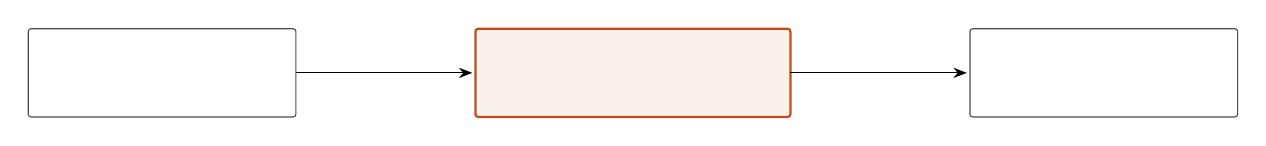
\begin{tikzpicture}[x=0.2mm,y=-0.2mm]
% 箱は左上の角と幅、高さで置き、文字は M（中央）、S（左寄せ）、E（右寄せ）の基線で置く
\draw[rb] (16,20) rectangle ++(170,56);
\node[tb,M] at (101,44) {〈入力〉};
\node[ts,M] at (101,62) {〈補足〉};
\draw[ro] (300,20) rectangle ++(200,56);
\node[tb,M] at (400,44) {〈本報告で作ったもの〉};
\node[ts,M] at (400,62) {〈補足〉};
\draw[rb] (614,20) rectangle ++(170,56);
\node[tb,M] at (699,44) {〈出力〉};
\node[ts,M] at (699,62) {〈補足〉};
\draw[arr] (186,48) -- (298,48);
\node[ts,M] at (242,40) {〈流れるもの〉};
\draw[arr] (500,48) -- (612,48);
\node[ts,M] at (556,40) {〈流れるもの〉};
\end{tikzpicture}
\caption{〈この図が示す主張を 1 文。続けて、読み方の補足。〉}
\label{fig:overview}
\end{figure*}

\subsection{本報告の内容と読み方}
\begin{itemize}
\item 〈貢献 1〉（\ref{sec:method} 章）
\item 〈貢献 2〉（\ref{sec:results} 章）
\end{itemize}
〈分野に不慣れなら何章から、成果物だけ知りたければ何章を読むか。〉

%% =========================================================
\section{予備知識}\label{sec:prelim}
〈読み手が知らない概念を、この素材に出てくる実際の名前を例に説明する。不要なら章ごと消す。〉
\begin{itemize}
\item 〈用語〉: 〈1〜2 文の説明〉
\end{itemize}

%% =========================================================
\section{システム構成}\label{sec:system}
〈ハードウェアとソフトウェアの構成。部品の一覧は表にする。〉

\begin{table}[tb]
\caption{〈表の内容〉}\label{tab:parts}
\footnotesize\sffamily
% セルには短い語句だけを置く。文は本文に書く（build.sh はセルの中の「。」で失敗する）
\begin{tabularx}{\columnwidth}{@{}l Y Y@{}}
\toprule
要素 & 仕様 & 役割 \\
\midrule
〈要素〉 & 〈仕様〉 & 〈役割〉 \\
〈要素〉 & 〈仕様〉 & 〈役割〉 \\
\bottomrule
\end{tabularx}
\end{table}

%% =========================================================
\section{手法}\label{sec:method}
〈どうやったか。式は番号を振り、記号はすべて本文で定義する。〉
\begin{equation}
w = \frac{\sigma_a^2}{\sigma_a^2 + \sigma_b^2}
\label{eq:weight}
\end{equation}
〈式 (\ref{eq:weight}) の各記号の意味と、係数の出どころ。〉

%% =========================================================
\section{実験と結果}\label{sec:results}
〈条件、結果の表と図、読み取れること。数値はすべて出典のある値にする。〉

\begin{figure}[tb]
\centering
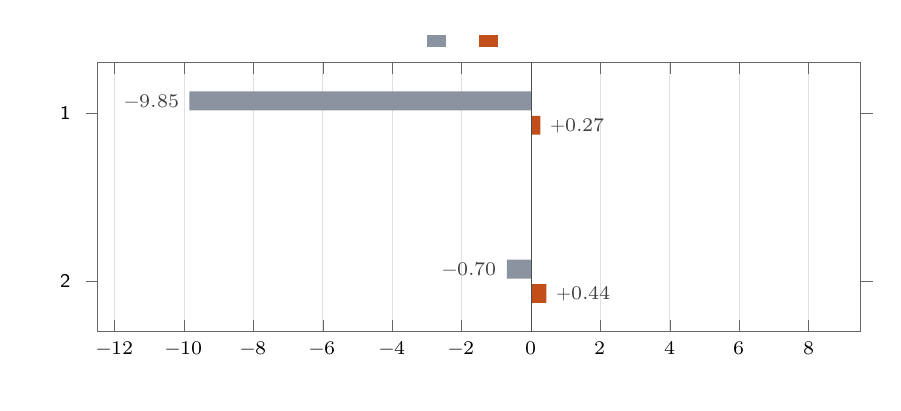
\begin{tikzpicture}
\begin{axis}[
  xbar,
  width=0.93\columnwidth, height=5cm,
  bar width=2.4mm,
  xmin=-12.5, xmax=9.5,
  ytick={1,2},
  % 上から並べたい順と逆に y を振る（上の項目ほど大きい y）
  yticklabels={〈項目 2〉,〈項目 1〉},
  yticklabel style={font=\sffamily\scriptsize,align=right},
  xticklabel style={font=\sffamily\scriptsize},
  enlarge y limits=0.3,
  xmajorgrids, grid style={black!12},
  axis line style={black!60}, tick style={black!60},
  xlabel={\sffamily\scriptsize 〈量（単位）〉},
  legend style={at={(0.5,1.03)},anchor=south,legend columns=2,draw=none,font=\sffamily\scriptsize},
  legend image code/.code={\fill[#1] (0cm,-0.8mm) rectangle (2.4mm,0.8mm);},
  % 正負で左右に振り分けるには、メタ値を数値（x）で渡す
  point meta=x,
  nodes near coords={\pgfmathprintnumber[fixed,fixed zerofill,precision=2,showpos]{\pgfplotspointmeta}},
  nodes near coords align=horizontal,
  every node near coord/.append style={font=\sffamily\scriptsize,text=black!75},
  reverse legend,
]
% 後に描いた系列ほど各グループの上に並ぶ。凡例は reverse legend で上からの順に戻す
\addplot[fill=ours,draw=none] coordinates {(0.27,2) (0.44,1)};
\addplot[fill=seriesA,draw=none] coordinates {(-9.85,2) (-0.70,1)};
\draw[black!70] (axis cs:0,0.5) -- (axis cs:0,2.5);
\legend{〈提案〉,〈比較〉}
\end{axis}
\end{tikzpicture}
\caption{〈この図が示す主張を 1 文。〉}
\label{fig:result}
\end{figure}

比べる数値は図にし、正確な値を引く必要があるものだけを表\ref{tab:numbers} のように表にする。

\begin{table}[tb]
\caption{〈表の内容〉。単位は見出しに書く}\label{tab:numbers}
\footnotesize\sffamily
% S 列は小数点の位置でそろえる。table-format は「符号、整数の桁数、小数の桁数」
\begin{tabular}{@{}l S[table-format=2.1] S[table-format=1.2] S[table-format=-1.2]@{}}
\toprule
〈条件〉 & {〈量 A〉 [\%]} & {〈量 B〉 [cm]} & {〈差〉 [°]} \\
\midrule
〈条件 1〉 & 10.8 & 0.60 & -6.00 \\
〈条件 2〉 & 0.0 & 0.61 & 3.50 \\
\bottomrule
\end{tabular}
\end{table}

%% =========================================================
\section{考察}\label{sec:discussion}
〈結果から何が言えるか、限界、検証の進め方で役立ったこと。〉

%% =========================================================
\section{現状と今後}\label{sec:status}
\subsection{成果物の一覧}
状態の「実機」は動作と数値を確かめたもの、「実装」は実装したが結果を記録していないものを表す。
\begin{table*}[tb]
\caption{成果物と状態}\label{tab:status}
\footnotesize\sffamily
\begin{tabularx}{\textwidth}{@{}Y Y l@{}}
\toprule
成果物 & 場所 & 状態 \\
\midrule
〈成果物〉 & \code{PATH} & 実機 \\
〈成果物〉 & \code{PATH} & 実装 \\
\bottomrule
\end{tabularx}
\end{table*}

\subsection{作業中の変更}
〈未コミットの変更。結果が無いことも書く。〉

\subsection{残る課題}
\begin{itemize}
\item 〈課題〉
\end{itemize}

%% =========================================================
\begin{thebibliography}{99}\small
\bibitem{ref1} 〈著者〉. 〈題〉. \textit{〈誌名〉}, 〈巻（号）〉, 〈年〉.
\bibitem{ref2} 〈名前〉. \url{https://example.com/}
\end{thebibliography}

%% =========================================================
\appendix
\section{用語の対応}\label{app:terms}
〈素材が独自の呼び方を使うときだけ、一般の用語との対応表を置く。〉

\end{document}
